\documentclass{svproc}

\usepackage{url}
\usepackage{hyperref}
\usepackage{graphicx}
\usepackage{multicol}
\usepackage{footmisc}
\usepackage{listings}
\usepackage{xcolor}

\def\UrlFont{\rmfamily}

\lstset { %
    language=C++,
    backgroundcolor=\color{black!5}, % set backgroundcolor
    basicstyle=\footnotesize,% basic font setting
}

\hypersetup{
    colorlinks=true,
    urlcolor=blue
}

\begin{document}
\mainmatter

\title{
Chess Mentor \\
Backend Technical Report} 
\author{Group B3}

\institute{
Artificial Intelligence, \\
Faculty of Computer Science, \\
Alexandru Ioan Cuza University, Iasi, Romania}

\maketitle

\begin{abstract}
This paper contains the detailed presentation on Chess Mentor, an artificial intelligence that can guide you trough a game of chess, providing moves from different strategies at each step and insightful commentaries at the end of each game so you can become better.
\keywords{backend, chess, artificial intelligence, mentor}
\end{abstract}

\section{Researching programming languages}

\subsubsection{•}
When deciding the programming language used for this project, the language speed played a key factor in our choice because the algorithms we use require a lot of calculations.

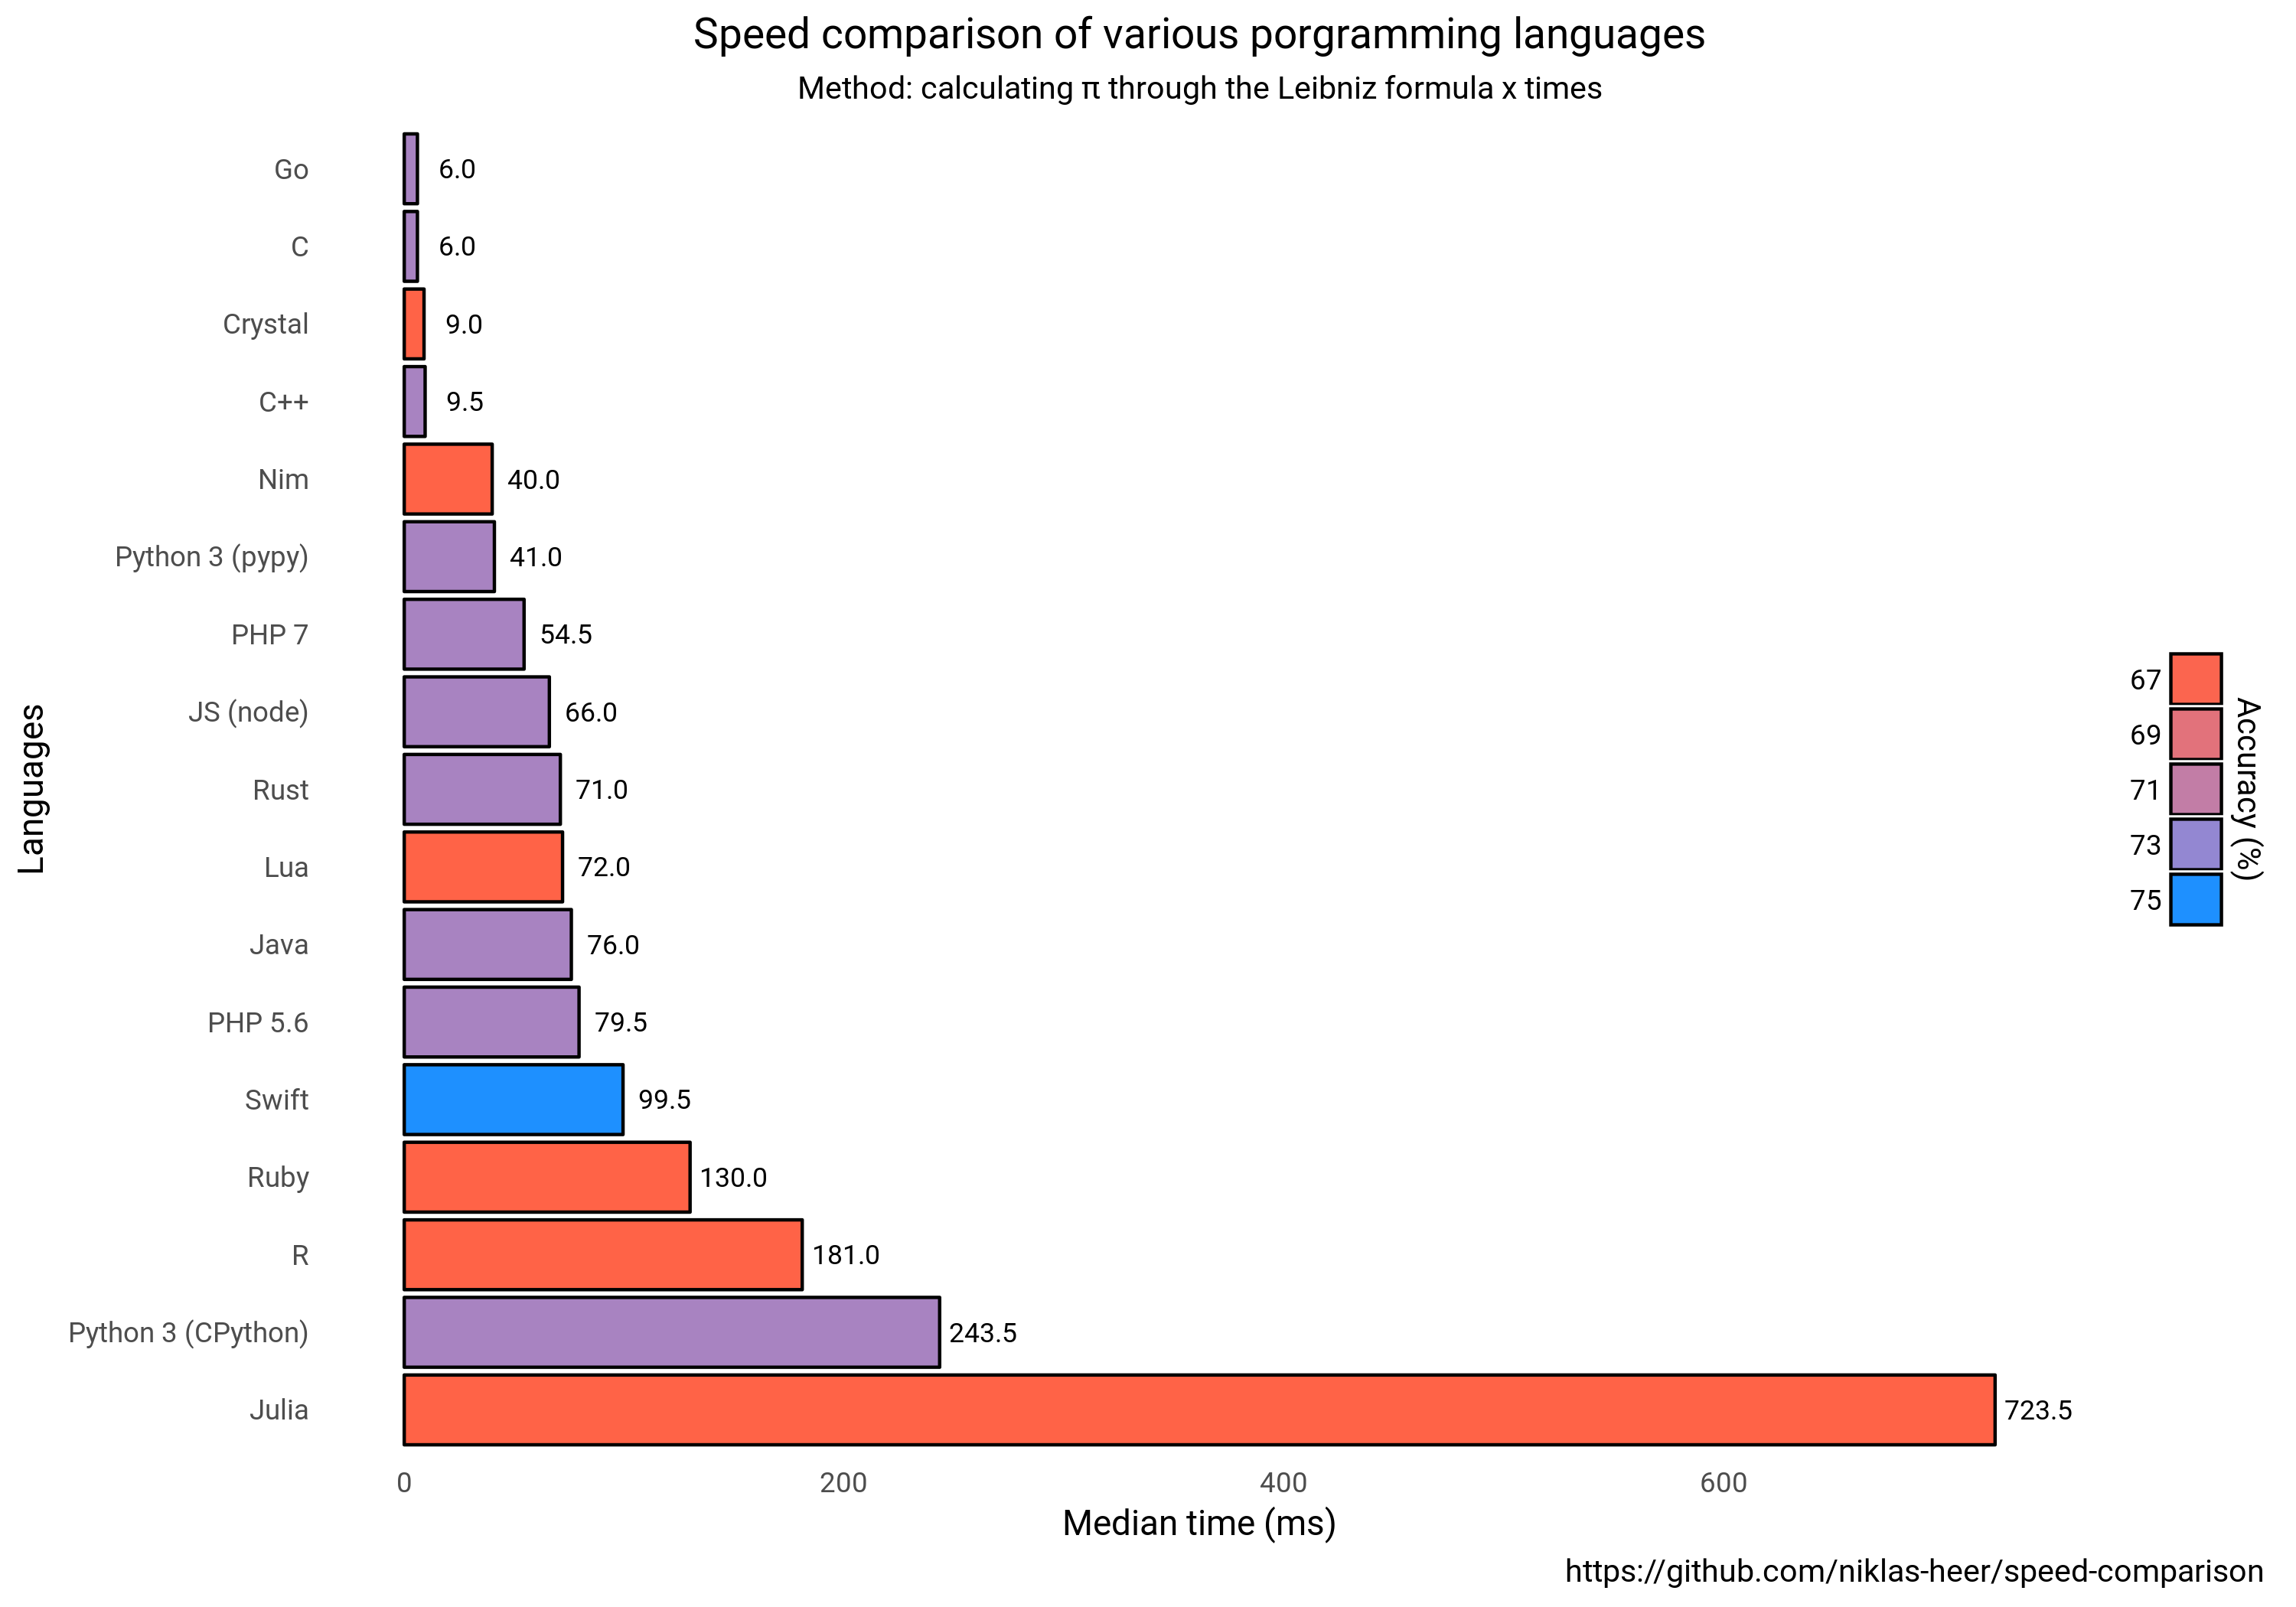
\includegraphics[scale=0.5]{programming-languages-speed}

\subsubsection{•}
This chart is comparing Julia - JIT, R - interpreted, Python - interpreted (CPython), Ruby - interpreted, Swift - compiled (in this test interpreted due to Linux Swift limitations), Java - compiled, VM, Rust - compiled, Javascript using Node.js - interpreted, JIT, Lua - interpreted, Nim - compiled, PHP - interpreted, C++ - compiled, Crystal - compiled, Go - compiled, C - compiled languages on calculating Leibniz formula for π. On a quick look we notice that Python has a very good median time. The faster languages are only C, C++, Nim, Crystal and Go.

\subsubsection{•}
Even if Python is a general purpose language, often used for things other than data science and analysis, some things make it very useful for working with data.

\subsubsection{•}
Libraries give users essential functionality when managing data. Python has a lot of popular and useful libraries for machine learning. After you get familiarized with them, they become a staple in a machine learning developing kit.

\bigskip

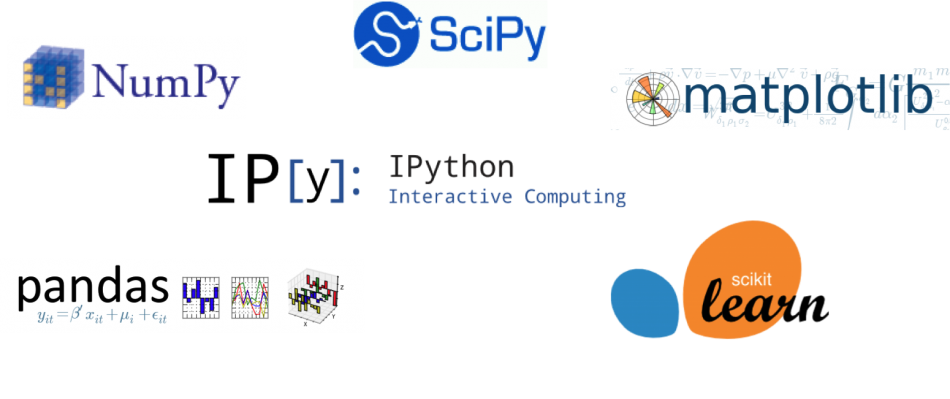
\includegraphics[scale=0.33]{python-machine-learning-libraries}

\subsubsection{•}
Trough these popular libraries we can find:
\begin{itemize}
	\item Pandas: used for data manipulation and analysis. It’s used frequently on data preparation and munging. It is added recently to python and founds usage by data scientists. 
	\item Scikit-learn: this library for machine learning has been built on NumPy, SciPy and matplotlib, it contains a lot of usefull tools for maching learning, clustering, regression, classification and reduction.
	\item Seaborn: Used for data visualization, mostly statistical. It is based on matplotlib and aims to make attractive graphics.
	\item and many more!
\end{itemize}

\pagebreak

\subsubsection{•}
One more thing we kept in mind, was that we needed a programming language that is easy to pick up. Our project has enough difficulty in understanding (business) so we don’t want to add extra problems on understanding the language we decide upon. According to a survey in which hundreds of developers from the US participated, women and men, the results are:

\begin{enumerate}
  \item HTML (13.3\%)
  \item Python (9\%)
  \item Javascript (6.2\%)
  \item PHP (4.9\%)
  \item Java (4.6\%)
  \item R (4.4\%)
  \item Shell (4.4\%)
  \item Ruby (4.1\%)
  \item Erlang (3.8\%)
  \item Go (3.6\%)
\end{enumerate}

\subsubsection{•}
This survey confirms that Python is a language with high readability and very simple syntax. It’s being surpassed by only HTML which is a markup-language. 



\section{Environment}

\subsubsection{•}
The project's backend was developed under Windows 10 Pro 64bit, using Python 3.7.0. 

\subsubsection{•}
The only framework used for exposing the API via HTTP is Flask (\url{http://flask.pocoo.org/}), a BSD licensed microframework for Python based on Werkzeug and Jinja 2.

\section{Architecture}

\subsubsection{•}
The backend serves static HTML/CSS/JS content for the '/' path and exposes 3 more paths, all 3 returning JSONs: 

\begin{enumerate}
  \item '/strategies' which returns an array of strings representing the names of the available strategies
  \item /moves?strategy=STRATEGY \& fen=FEN' which returns the move a certain strategy does from a specific board state
  \item '/commentary?game=GAME' which returns a commentary for the given game
\end{enumerate}

\section{Chess strategies}

\subsubsection{•}
For move recommendations we used a series of classical AI game algorithms like minmax or negamax combined with already existing chess engines like Stockfish.

\subsection{Minmax}

\subsubsection{•}
Minimax is a decision-making algorithm , typically used in a turn-based, two player games. The goal of the algorithm is to find the best move for the player. To do so, we can just choose the node with best evaluation score. To make the process smarter, we can also look ahead and evaluate potential opponent’s moves.

\subsubsection{•}
In this algorithm, the recursive tree of all possible moves is explored to a given depth, and the position is evaluated at the ending “leaves” of the tree.

\subsubsection{•}
After that, we return either the smallest or the largest value of the child to the parent node. That is, we try to either minimize or maximize the outcome at each level, based of course on whether  is black or white to move.

\begin{center}
  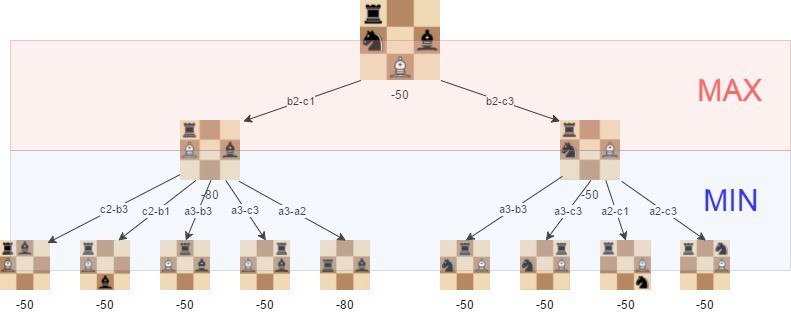
\includegraphics[scale=0.4]{minmax}
\end{center}

\subsubsection{•}
The picture above shows the visualization of the minimax algorithm in an artificial position. We can note that the best move for white is B2C3 ,because that guarantees a further position where the evaluation is -50.

\subsubsection{•}
The effectiveness of the minimax algorithm is heavily based on the search depth we can achieve.Therefore we’ll get into Alpha-beta pruning.


\subsection{Alpha-beta pruning}

\subsubsection{•}
Alpha-beta pruning is an optimization method to the minimax algorithm that allows us to disregard some branches in the search tree. This helps us evaluate the minimax search tree much deeper, while using the same resources.

\pagebreak

\subsubsection{•}
The alpha-beta pruning is based on the situation where we can stop evaluating a part of the search tree if we find a move that leads to a worse situation than a previously discovered move. It does not influence the outcome of the minimax algorithm  —  it only makes it faster. The alpha-beta algorithm also is more efficient if we happen to visit first those paths that lead to good moves.

\begin{center}
  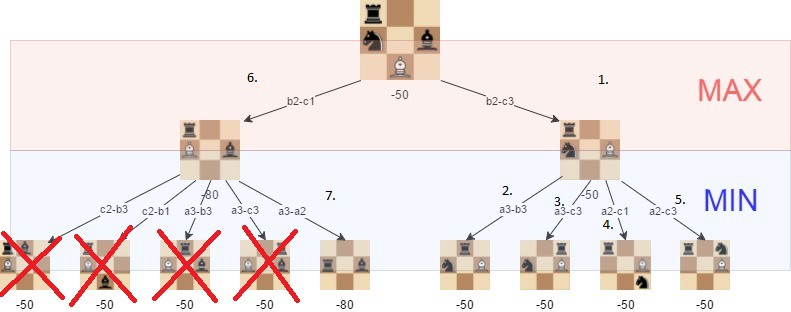
\includegraphics[scale=0.4]{alpha-beta-pruning-1}
\end{center}

\subsubsection{•}
We can notice the positions we do not need to explore if alpha-beta pruning issued and the tree is visited in the described order .That means we no longer have to go more in depth on the disregarded branches and that clearly will improve the execution time.

\begin{center}
  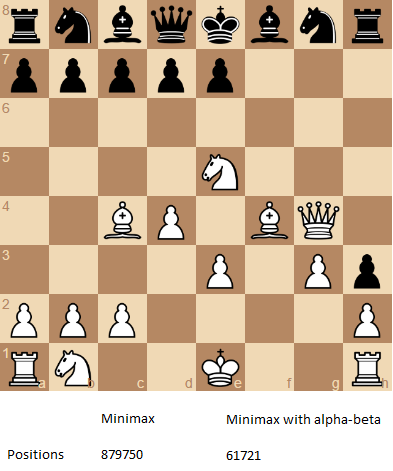
\includegraphics[scale=0.6]{alpha-beta-pruning-2}
\end{center}

\subsubsection{•}
The number of positions that are required to evaluate if we want to perform a search with depth of 4 and the “root” position is the one that is shown.

\subsection{IDS}

\subsubsection{•}
Iterative deepening search (IDS) has been adopted as the basic time management strategy in depth-first searches, but has proved surprisingly beneficial as far as move ordering is concerned in alpha-beta pruning and its enhancements. It has been noticed, that even if one is about to search to a given depth, that iterative deepening is faster than searching for the given depth immediately. This is due to dynamic move ordering techniques such as; PV-, hash- and refutation moves determined in previous iteration(s), as well the history heuristic.

\subsubsection{•}
It works as follows: the program starts with a one ply search, then increments the search depth and does another search. This process is repeated until the time allocated for the search is exhausted. In case of an unfinished search, the program always has the option to fall back to the move selected in the last iteration of the search. Yet if we make sure that this move is searched first in the next iteration, then overwriting the new move with the old one becomes unnecessary. This way, also the results from the partial search can be accepted - though in case of a severe drop of the score it is wise to allocate some more time, as the first alternative is often a bad capture, delaying the loss instead of preventing it. Iterative deepening, using a transposition table, embed the depth-first algorithms like alpha-beta into a framework with best-first characteristics.

\subsection{Negamax}

\subsubsection{•}
Negamax, a common way of implementing Minimax and derived algorithms. Instead of using two separate subroutines for the Min player and the Max player, it passes on the negated score due to following mathematical relation: \\ max(a, b) == -min(-a, -b).

\pagebreak

\subsection{Stockfish - ENGINE}

\begin{center}
  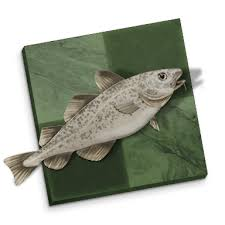
\includegraphics[scale=0.6]{stockfish}
\end{center}

\subsubsection{•}
Stockfish is a free and open-source UCI chess engine, available for various desktop and mobile platforms. It is developed by Marco Costalba, Joona Kiiski, Gary Linscott and Tord Romstad, with many contributions from a community of open-source developers.

\subsubsection{•}
Stockfish is consistently ranked first or near the top of most chess-engine rating lists and is the strongest open-source chess engine in the world. It won the unofficial world computer chess championships in season 6 (2014), season 9 (2016), season 11 (2018), season 12 (2018), and season 13 (2018). It finished runner-up in season 5 (2013), season 7 (2014) and season 8 (2015). Stockfish is derived from Glaurung, an open-source engine by Romstad.

\subsubsection{•}
Stockfish implements an advanced alpha-beta search and uses bitboards. Compared to other engines, it is characterized by its great search depth, due in part to more aggressive pruning and late move reductions. 

\subsection{Hermann - ENGINE}

\subsubsection{•}
Hermann, a Chess Engine Communication Protocol and UCI compliant chess engine by Volker Annuss, able to play Chess960. Hermann is Arena partner engine, participating the Chess960CWC 2005, Chess960CWC 2006, CPT 2009, CPT 2010 and various Dutch Open Computer Chess Championships and International CSVN Tournaments, third place at ICT 2009.

\subsubsection{•}
Hermann uses bitboards as basic data structure, determines sliding piece attacks with fixed shift magic bitboards, and applies neural networks for material evaluation and timing. In 2011, Volker Annuss confirmed his soft spot for his engine names associated with the legacy of romantic German nationalism by calling Hermann's completely restructured successor with its Latinised name Arminius. In Germany, Arminius was rechristened Hermann (Heer Mann - army man) by Martin Luther, and he became an emblem of the revival of German nationalism fueled by the Napoleon wars in the 19th century.

\subsection{Ruffian - ENGINE}

\subsubsection{•}
Ruffian is a strong chess engine that can be loaded as a winboard or 
UCI engine. Ruffian supports most winboard (version 1 and 2) and UCI
options. The program has been developing in C language since 1998. It has used various known techniques like bitboards (combines it with 8x8 representation), null move, prunning, extensions. The opening library is not of high quality and sophisticated, it was automatically generated from a small PGN database.

\subsection{Rybka - ENGINE}

\begin{center}
  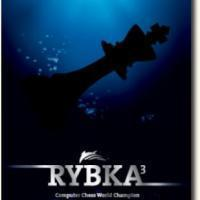
\includegraphics[scale=0.5]{rybka}
\end{center}

\subsubsection{•}
Rybka is a chess engine designed by Vasik Rajlich, International Master. \\ Rybka was one of the top-rated engines on chess engine rating lists and has won many computer chess tournaments and it uses a bitboard representation and is an alpha-beta searcher (search algorithm that seeks to decrease the number of nodes that are evaluated by the minimax algorithm in its search tree). It uses very aggressive pruning, leading to imbalanced search trees. The details of the evaluation function of this engine are unknown.


\subsection{SOS - ENGINE}

\subsubsection{•}
SOS, a chess program developed and written by Rudolf Huber in the C programming language. In its early times in the mid 90s, SOS running on various platforms and operating systems had an own futuristic graphical user interface. SOS supported the Chess Engine Communication Protocol, was available as Young Talent by ChessBase running under Fritz6 GUI, and since Rudolf is co-designer of the protocol, it finally changed to UCI, and is a Partner Chess Engine of Arena (free Graphical User Interface for Chess Engine Communication Protocol and UCI compatible engines running under Windows). 

\subsubsection{•}
SOS uses depth first minimax tree search with quiescence search, alpha-beta enhancement, minimal window search and null-move pruning. To improve the search efficiency, the history heuristic and a trans-positional table is used. The evaluation parameters are dynamic and continuously updated during tree search. SOS's weakest part is probably endgame knowledge. SOS actively plays a wide range of openings, but most of those lines are not very deep. With auto-play games against itself, the opening book is tuned to favor those lines which harmonize with SOS's style of play. 


\subsection{Spike - ENGINE}

\begin{center}
  
\includegraphics[scale=1]{spike}
\end{center}

\subsubsection{•}
Spike is a chess engine developed since spring 2004. It is developed  
from the scratch but uses many ideas already tested on our two other 
engines: Cheetah and IceSpell.

\subsubsection{•}
Spike is a typically brute force program with a pvs algorithm. The board structure is a kind of 0x88 but has an additional border above and below the chess-field. The board has 14x16 fields to make move generation as easy as possible. With the version 1.0 Spike got some new pruning rules, 
the biggest prunings are Nullmove (for a long time already), History 
(Version 1.0) and Futility (Version 1.1).

\subsubsection{•}
The eval checks pawn structure (double, isolated, backward, passed, 
connected and combinations of them), king security, pawn shield, 
mobility, piece attack/defence, rook on open lines, rook or queen on 
7-th or 8-th row, knight and bishop position, trapped rooks and knights 
outposts supported by own pawns that cannot be attacked by opponents 
pawns.

\end{document}
